\justifying
\begin{problem}{1}
	Пліт, що має форму прямокутника зі сторонами $5$м $\times 10$ м, рухається вночі за течією річки зі швидкістю $0.5 \dfrac{\text{м}}{\text{с}}$. Вздовж краю плоту ходить людина з гасовою лампою зі швидкістю $1 \dfrac{\text{м}}{\text{c}}$. Намалюйте траєкторію руху ліхтарика відносно землі за $30$ секунд руху (саме вздовж цієї лінії буде рухатись світлова пляма, якщо саостерігати за місцевістю згори). 
\end{problem}

\begin{problem}{1}
	Частинка рухається в одній площині. По графікам залежності від часу проекцій швидкості частинки $v_x$ та $v_y$ побудуйте траєкторію частинки, якщо $x(0) = 2$ м, $y(0) = 1$ м.
	
	\begin{figure}[h!]
		\begin{tikzpicture}
			\begin{axis}[xlabel = {$t$},
			ylabel = {$v_x, \text{м/с}$}]
			\addplot coordinates {
				(0,-1) (1,-1) (1,1) (2,1) (2,0) (3,0) (3, -1) (4,-1) (4,0)
			};
			\end{axis}
		\end{tikzpicture}
		\hfill
		\begin{tikzpicture}
		\begin{axis}[xlabel = {$t$},
		ylabel = {$v_y, \text{м/с}$}]
		\addplot coordinates {
			(0,0) (1,0) (1,1) (3,1) (3,0) (3,0) (4, 0)
		};
		\end{axis}
		\end{tikzpicture}
		\caption{До задачі \arabic{assigments}.\arabic{problems}}
	\end{figure}
\end{problem}

\begin{problem}{1}
	Рухаючись до табору, Михайло проїхав першу половину шляху зі швидкістю $v_1 = 60~ \dfrac{\text{км}}{\text{год}}$. Половину часу, що залишилось, проїхав зі швидкістю $v_2 = 15~\dfrac{\text{км}}{\text{год}}$, а останню ділянку шляху зі швидкістю $v_3 = 45~ \dfrac{\text{км}}{\text{год}}$. Чому дорівнює середня швидкість автомобіля на всьому шляху?
\end{problem}


\begin{problem}{2}
	Ескалатор підіймає стоячу людину з час $t_1 = 1$ хв; якщо ескалатор не рухається, то людина підіймається ескалатором за $t = 3$ хв (проходить ту саму відстань). Скільки часу буде підійматись людина, яка буде рухатись працюючим ескалатором?
\end{problem}

\begin{problem}{\label{balls}}
	Дві кульки (червона та зелена) рухаються прямолінійними траєкторіями (див. рис. \ref{2_balls}) зі швидкостями: $v_1 = 1.5 ~\dfrac{\text{м}}{\text{c}}$ - зелена, $v_2 = 1,2~\dfrac{\text{м}}{\text{c}}$. Знайти відносну швидкість другої кульки відносно першої.
	\begin{figure}[h!]
		\centering
		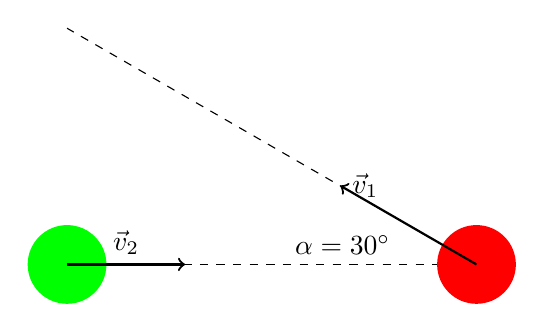
\begin{tikzpicture}
		\draw [dashed] (5.2,0) -- (0,3);
		\draw [dashed] (0,0) -- (5.2,0);
		
		\fill[green] (0,0) circle (0.5cm);
		\fill[red] (5.2,0) circle (0.5cm);
		
		\draw [->, thick] (5.2,0) -- (3.47, 1);
		\node [right] at (3.5, 1) {$\vec{v}_1$};
		
		\draw [->, thick] (0,0) -- (1.5, 0);
		\node [above] at (0.75,0) {$\vec{v}_2$};
		
		\node [above] at (3.5, 0) {$\alpha = 30^{\circ}$};
		\end{tikzpicture}
		\caption{До задачі \arabic{assigments}.\arabic{problems}}
		\label{2_balls}
	\end{figure}
	
\end{problem}

\begin{problem}{2}
	Неочікувано в кінці березня пішов сніг! Але на вулиці в цей час гуляли Стас та Марина. Марина йшла до Стасу зі швидкістю $v$, а Стас стояв нерухомо і помітив, що швидкість сніжинок дорівнює $u$ і падають вони перпендикулярно до поверхні землі (концентрація сніжинок однакова у будь-якій точці простору). Вважаючи, що голови у друзів - це дві однакові сфери, знайти, на яку з голів падає більше сніжинок? у скільки разів?
\end{problem}

\begin{problem}{\label{2_lines}}
	Дві прямі перетинаються під кутом $\alpha$ (див. рис. \ref{to_2_lines}), рухаються перпендикулярно самим собі зі швидкостями $v_1$ та $v_2$. Знайдіть швидкість $v$ точки перетину прямих
	
	\begin{figure}[h!]
		\centering
		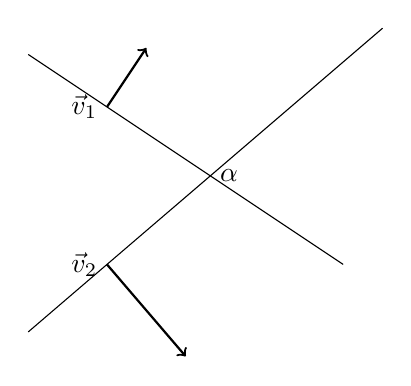
\begin{tikzpicture}
			\draw [thin] (-1,1.6667) -- (3,-1);
			\draw [thin] (-1,-1.857) -- (3.5, 2);
			
			\draw [->, thick] (0, -1) -- (1,-2.167);
			\draw [->, thick] (0, 1) -- (0.5,1.75);
			
			\node [left] at (0,1) {$\vec{v}_1$};
			\node [left] at (0,-1) {$\vec{v}_2$};
			 
			\node [right] at (1.3125,0.125) {$\alpha$};
		\end{tikzpicture}
		
		\caption{До задачі \arabic{assigments}.\arabic{problems}}
		\label{to_2_lines}
	\end{figure}
\end{problem}

\textbf{Задачі для самостійного розв'язання}
\begin{problem}{1}
	Якісні питання:
	\begin{enumerate}
		\item Яка траєкторія руху точок винта мотороного літака відносно пілота?  відносно землі?
		\item Біля нерухомого автомобіля проїзжджає колона вантажівок, які рухаються з однаковою швидкістю. Чи рухається кожна вантажівка відносно автомобіля? Чи рухається вантажівка відносно іншої вантажівки? Чи рухається автомобіль відносно вантажівки
		\item З центру горизонтально розташованого диску, який обертаэться, по його поверхні запустили кульку. Якими будть траєкторії кулькуи відносно Землі та відносно диска?
		\item Чому краплі дощу у безповітряну погоду залишають похилі прямі полоси на склі вагону потяга, який рівномірно рухається?
	\end{enumerate}
\end{problem}

\begin{problem}{3}
	Коли машина Тараса Дмитровича ненароком ламається він зазвичай кладе її собі на плечі та продовжує рух, але повільніше: коли Тарас Дмитрович на машині їх швидкість становить $120~\dfrac{\text{км}}{\text{год}}$, а коли машина на Тарасі Дмитровичі -- $30~\dfrac{\text{км}}{\text{год}}$. Чому дорівнює їх середня швидкість, якщо 
	\begin{enumerate}
		\item Тарас Дмитрович їде половину шляху а потім несе машину
		\item Тарас Дмитрович їде половину часу а потім несе машину
	\end{enumerate}
\end{problem}

\begin{problem}{5}
	Людина, яка спускається по працюючому на спуск ескалаторі, витрачає на спуск 1 хв, Якщо людина буде йти вдвічі швидше, то витратить на 15 с менше. Скільки часу людина буде спускатись стоючи на працюючому есклалторі?
\end{problem}

\begin{problem}{2}
	Двома дорогами, що перетинаються під прямим кутом рівномірно рухаються автомобілі, швидкості яких дорівнюють $72$ та $54~\dfrac{\text{км}}{\text{год}}$. Знайдіть відносну швидкість одного відносно іншого
\end{problem}

\begin{problem}{3}
	По паралельних коліях назустріч рухаються два потяги: пасажирський завдовжки $300$ м зі швидкістю $60~\dfrac{\text{км}}{\text{год}}$ і вантажний зі швидкістю $40 ~\dfrac{\text{км}}{\text{год}}$. Машиніст вантажного потягу виміряв, що вантажний потяг проїжджає повз нього за $21.6$ с. Визначіть відстань від місця зустрічі потягів до місця розходження останніх вагонів.
\end{problem}

\begin{problem}{3}
	За графіками залежності швидкості від часу побудуйте графіки залежності координати від часу. 
	\newpage
	\begin{figure}[h!]
		\begin{minipage}[h!]{0.45\linewidth}
			а) \\
			\begin{tikzpicture}
			\begin{axis}[title = {$x(0) = 2 \text{м}$}, xlabel = {$t$},
			ylabel = {$v, \text{м/с}$},grid=both, grid style={dashed, cyan},  minor xtick={-10,-8,...,10,12},minor grid style={dotted,red, line width=0.2pt}]
			\addplot coordinates {
				(-10,0) (-6,0) (-6,4) (-2,4) (-2,1) (2,1) (2,-2) (10,-2) (10, 0) (12,0)
			};
			\end{axis}
			\end{tikzpicture}
		\end{minipage}
		\hfill
		\begin{minipage}[h!]{0.45\linewidth}
			б)
			
			\begin{tikzpicture}
			\begin{axis}[title = {$x(0) = -1 \text{м}$}, xlabel = {$t$},
			ylabel = {$v, \text{м/с}$},grid=both, grid style={dashed, cyan},  minor xtick={-10,-8,...,10,12},minor grid style={dotted,red, line width=0.2pt}]
			\addplot coordinates {
				(-8,-2) (-8,2) (-6,2) (-6,-2) (-4,-2)  (-4,2) (-2, 2) (-2,-2) (0,-2) (0,-2) (0,2) (2,2) (2,-2) (4,-2) (4,2) (6,2) (6,-2) (8,-2) (8,2) (10,2)
			};
			\end{axis}
			\end{tikzpicture}
		\end{minipage}
		
		\begin{minipage}[h!]{0.45\linewidth}
			в) \\
			\begin{tikzpicture}
			\begin{axis}[title = {$x(0) = -1 \text{м}$}, xlabel = {$t$},
			ylabel = {$v, \text{м/с}$},grid=both, grid style={dashed, cyan},  minor xtick={-10,-8,...,10,12},minor grid style={dotted,red, line width=0.2pt}]
			\addplot coordinates {
				(-8,-1) (-8,3) (-6,3) (-6,-1) (-4,-1)  (-4,3) (-2, 3) (-2,-1) (0,-1) (0,3) (2,3) (2,-1) (4,-1) (4,3) (6,3) (6,-1) (8,-1) (8,3) (10,3)
			};
			\end{axis}
			\end{tikzpicture}
		\end{minipage}
		\caption{До задачі \arabic{assigments}.\arabic{problems}}
	\end{figure}
\end{problem}
